\documentclass[12pt]{article}
\usepackage[]{algorithm2e}
\usepackage{amsmath, verbatim}
\usepackage{amssymb}
\usepackage[margin=1in]{geometry}
\usepackage{tikz}
\usetikzlibrary{decorations.markings}
\usetikzlibrary{decorations.pathreplacing}
\allowdisplaybreaks
\usepackage{chngcntr}
\counterwithin{figure}{section}
\usepackage{authblk}
\usepackage{amsthm}
\usepackage{mathtools} % for alignment of pmatrix in Example 2.4
%\pagenumbering{gobble}
\newcommand{\E}{\mathbf{E}}
\newcommand{\R}{\mathbb{R}}
\newcommand{\rr}{\mathbb{R}}
\newcommand{\N}{\mathbb{N}}
\newcommand{\QQ}{\mathbb{Q}}
\newcommand{\C}{\mathbb{C}}
\newcommand{\x}{\mathbf{x}}
\newcommand{\w}{\mathbf{w}}
\newcommand{\e}{\mathbf{e}}
\newcommand{\ba}{\mathbf{a}}
\newcommand{\g}{\mathbf{g}}
\newcommand{\calF}{\mathcal{F}}
\newcommand{\calS}{\mathcal{S}}
\newcommand{\calB}{\mathcal{B}}
\newcommand{\calm}{\mathcal{M}}
\newcommand\norm[1]{\left\lVert#1\right\rVert}
\DeclareMathOperator{\tr}{\mathrm{tr}}

\title{Coalescent-based phylogenetic tree reconstruction from $k$-mers: plan for Simulation Batch 1}
\author{Chris Durden}
\author{Seth Sullivant}
\affil{Department of Mathematics, North Carolina State University}

\newtheorem{theorem}{Theorem}[section]
\newtheorem{lemma}[theorem]{Lemma}
\newtheorem{proposition}[theorem]{Proposition}
\newtheorem{corollary}[theorem]{Corollary}

\theoremstyle{definition}
\newtheorem{definition}[theorem]{Definition}
\newtheorem{remark}[theorem]{Remark}
\newtheorem{example}[theorem]{Example}

\begin{document}
\tikzset{middlearrow/.style={
        decoration={markings,
            mark= at position 0.5 with {\arrow{#1}} ,
        },
        postaction={decorate}
    }
}
\maketitle
%\begin{abstract}
%\end{abstract}

\section{Introduction}
We divide the simulation process into two parts: (1) the simulation of sequence data and (2) the reconstruction of trees from sequence data. Multiple methods, or sets of parameter values, for performing each part are described in the following two sections. For each combination of the methods and parameters described in these two sections, we perform parts (1) and then part (2) to complete entire simulation and reconstruction process.

\section{Simulation of sequence data}

To simulate sequence data, we start with a species tree on $n$ taxa.
We use k-mer frequencies from the simulated data to compute an average k-mer distance, which we compare to theoretical expectations.
In order to obtain precise estimates of the theoretical expectation, we need sequence data from many genes with independent gene trees.
We let $N$ denote the number of genes (from independent loci in the above sense).
We simulate datasets consisting of $N \in \{50,100,200\}$.

Simulations of sequence data are performed by first generating gene trees for each gene according to the coalescent process on the given species tree. 
The simulation of the coalescent process for each gene is controlled by the global population size parameter $\theta$, and the $2n-3$ branch length parameters of the species tree.
We focus on the case $n=5$, since this is the simplest case for which all of our identifiability results apply for any $k>1$.
To reduce the dimension of the parameter space of tree metrics, we consider trees parameterized by two values $t_a$ and $t_b$ as shown in the following diagram. To generate branch lengths for our species trees, we sample $(t_a,t_b)$ from $(0,\infty)^2$ by sampling the corresponding Jukes-Cantor distances uniformly from $[0,3/4)^2$. We then simulate gene trees for $\theta \in \{0.01, 0.05\}$.

\begin{center}
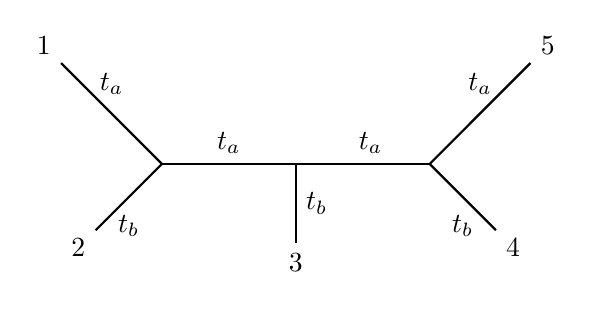
\begin{tikzpicture}[
        thick,
        level/.style={level distance=1.5cm},
        level 2/.style={sibling distance=3cm},
        level 3/.style={sibling distance=3cm}
    ]
    \coordinate
        child[grow=left, level distance=1.7cm]{
            child {
                node {$1$}
                edge from parent node [above=3pt] {$t_a$}
            }
            child[grow=south west, level distance=1.5cm] {
                node {$2$}
                edge from parent node [below=3pt] {$t_b$}
            }
            edge from parent node [above] {$t_a$}
        }
        child[grow=down, level distance=1.25cm]{
                node {$3$}
                edge from parent node [right] {$t_b$}
        }
        child[grow=right, level distance=0.2cm] {
        child  {
            child[grow=south east, level distance=1.5cm] {
                node {$4$}
                edge from parent node [below=3pt] {$t_b$}
            }
            child {
                node {$5$}
                edge from parent node [above=3pt] {$t_a$}
            }
            edge from parent
            node [above] {$t_a$}
        }
    };
\end{tikzpicture}
\end{center}

Once we have our gene trees, we simulate sequences using a mutation process operating on the gene tree. The mutation process may or may not include insertions and deletions (indels). The simulation of mutation is implemented in the program INDELible. The indel process operates on an initial sequence with length given by the parameter $m$. For point mutations, we use the Jukes-Cantor mutation process with substitution rate $\mu = 1$. We simulate sequences with and without an indel process. For simulations with an indel process, this process is controlled by the insertion and deletion rates, and by the distribution of the lengths of inserted and deleted segments. We set both the insertion and deletion rate parameter to a single value $\lambda \in \{0.01,0.05,0.1\}$, and we define the distribution of lengths using the Lavelette distribution with parameters $M=100$ and $a \in \{1.1, 1.5, 1.8\}$ (all values here match those in ARS2015).

%We use abbreviations to denote the various combinations of parameters defining the mutation processes. Show table...


\section{Reconstruction of trees given simulated sequence data}

For each combination of the coalescent and mutation process parameters above, we generate a set of simulated sequences. We then apply various tree reconstruction algorithms to each set of simulated sequences. We repeat this process multiple times to assess the frequency with which each reconstruction method reconstructs the original (true) tree.

The reconstruction methods we use are intended to compare our coalescent-based $k$-mer methods to previous alignment-free methods, and also to alignment-based methods. We thus devote subsections to each of these three types of methods.

Before describing these methods, we define some notation to be used to describe the methods based on computing averages of $k$-mer distances. Given sequence data, consisting of sequences $S_{i,g}$ for all $i \in [n], g \in [N]$, let $X_{i,g}$ be the $k$-mer count vectors for gene $g$. Let $m_{i,g}$ denote the length of the sequence of gene $g$ in species $i$, and let $\mu_{i,g} = (m_{i,g}-k+1)/4^k$. Let

\begin{align*}
    %D_{k,{ij},g} &= \frac{1}{2(m-k+1)}\sum_{g =1}^N \sum_{W \in \{A,T,C,G\}^k} (X^W_{i,g}-X^W_{j,g})^2,\\
    \overline{D}_{k,{ij}} &= \frac{1}{N}\sum_{g =1}^N \norm {\frac{X_{i,g}-\mu_{i,g}\mathbf{1}}{\sqrt{m_{i,g}-k+1}}-\frac{X_{j,g}-\mu_{j,g}\mathbf{1}}{\sqrt{m_{j,g}-k+1}}}.
%    \overline{D}_{k,{ij}} &= \frac{1}{N} \sum_{g \in [N]} D_{k,{ij},g}
\end{align*}
We call $\overline{D}_{k,{ij}}$ the normalized average $k$-mer distance between species $i$ and $j$.

The theoretical expectation of the average $k$-mer distance between two sequences under the Jukes-Cantor model with no indel process is given as a function of $\theta$ and the species divergence time $t$ by the following function.
\begin{align*}
    f_k(t,\theta) = 1-\frac{1}{4^k}\sum_{i=0}^{k} { k \choose i } \frac{3^{i+1} \exp(-4 t/3)}{3 + 8 \theta i}
\end{align*}

\subsection{Coalescent-based $k$-mer methods}

\subsubsection{Neighbor-Joining with coalescent and Jukes-Cantor model-based branch length estimates (CoalescentJCNJ)}
\begin{algorithm}[H]
    \KwData{$k_1, k_2 \in \mathbb{N}$, $\overline{D}_{k_1,ij}$, $\overline{D}_{k_2,ij}$ for all $i,j \in [n]$.}
 \KwResult{An unrooted phylogenetic tree $\hat{T}$}
% \lFor{$i<j$}{Let $\overline{D}_{k_1,{ij}}$ be the $k_1$-mer distance between sequences $i$ and $j$}
% \lFor{$i<j$}{Let $\overline{D}_{k_2,{ij}}$ be the $k_2$-mer distance between sequences $i$ and $j$}
 %\begin{align*}
            Compute the solution to the optimization problem $(\hat{t}_{12}, \ldots, \hat{t}_{n-1,n},\hat{\theta}) 
            = \operatorname*{arg\,min}\limits_{t,\theta} \sum_{i<j} \left([f_{k_1}(t_{ij},\theta)- \overline{D}_{k_1,ij}/2]^2 + [f_{k_2}(t_{ij},\theta) -\overline{D}_{k_2,ij}/2]^2\right).$\;

            Use Neighbor Joining to reconstruct a tree $\hat{T}$ from the estimated branch lengths $(\hat{t}_{12}, \ldots, \hat{t}_{n-1,n})$.\;
 %\end{align*}
 \caption{Coalescent-based Neighbor-Joining (CoalescentJCNJ) reconstruction method}
 \label{algorithm:NJcoalescent}
\end{algorithm}

\subsubsection{Least squares model fit method (CoalescentJCLS)}

Based on a result of our previous paper, the (unrooted) tree parameter is identifiable from the collection of expected $k$-mer distance among $5$-taxa, when $k>1$. This was proved by showing that there exists an invariant of the model $\calm_{k,T}$ which can be used distinguishes the trees. $\calm_{k,T}$ is the image of the parameterization map
\[
\phi_{k,T}  :  \rr^{2n -2}  \rightarrow   \rr^{n(n-1)/2}
\]
\[
(a_e : e \in E(T),  \theta)  \mapsto    \left(f_k\left( \prod_{e \in P(i,j)} a_e,  \theta\right)\right)_{1 \leq i < j \leq n}.
\]

Although we do not know the algebraic form of the model invariants, we know that they carve out different subspaces of $\R^{n \choose 2}$. Thus, with enough data, the tree $T$ which minimizes the distance between the image of $\calm_{k,T}$ and the data $(\overline{D}_{k,ij}/2 : i,j \in [n])$ will be the true tree, for most values of parameter. We use least squares to fit the model for each tree, and choose the tree which minimizes the least square distance.

\begin{algorithm}[H]
    \KwData{$k \in \mathbb{N}$, $\overline{D}_{k,ij}$ for all $i,j \in [n]$.}
 \KwResult{An unrooted phylogenetic tree $\hat{T}$}
% \lFor{$i<j$}{Let $\overline{D}_{k_1,{ij}}$ be the $k_1$-mer distance between sequences $i$ and $j$}
% \lFor{$i<j$}{Let $\overline{D}_{k_2,{ij}}$ be the $k_2$-mer distance between sequences $i$ and $j$}
 %\begin{align*}
           Compute the solution $\hat{T}$ to the optimization problem: $\hat{T} = \operatorname*{arg\,min}\limits_{T} \norm{ \phi_{k,T} - (\overline{D}_{k,ij}/2 : i,j \in [n]) }.$
 %\end{align*}
 \caption{Coalescent-based reconstruction method based on least squares model fitting (CoalescentJCLS)}
 \label{algorithm:5taxoninvariant}
\end{algorithm}

\subsubsection{Extensions of these methods to use more $k$-mer distance data}

We can modify the above methods to use $k$-mer distance data for $S_k \subset \N$, by estimating $\hat{T}$ separately for each $k \in S_k$ (or, in the case of NJ, for each pair $k_1,k_2 \in S_k$), and choosing the tree which is appears most frequently in the results.

\subsection{Other alignment-free methods}

The following reconstruction algorithms are derived from the simulation studies in ARS2015 Section 6. They are intended to emulate the methods used to generate Figures 6.6, 6.7, and 6.8.

\begin{algorithm}[H]
    \KwData{$k \in \mathbb{N}$, $\overline{D}_{k,ij}$ for all $i,j \in [n]$.}
 \KwResult{An unrooted phylogenetic tree $\hat{T}$}
% \lFor{$i<j$}{Let $\overline{D}_{k_1,{ij}}$ be the $k_1$-mer distance between sequences $i$ and $j$}
% \lFor{$i<j$}{Let $\overline{D}_{k_2,{ij}}$ be the $k_2$-mer distance between sequences $i$ and $j$}
 %\begin{align*}
 For each $i,j$ let 
 $\hat{t}_{ij} = -\frac{3}{4}\log\left(\frac{4}{3}\sqrt[k]{1 - \frac{\overline{D}_{k,ij}}{2}}-\frac{1}{3}\right)$

            Use Neighbor Joining to reconstruct trees from estimated branch lengths $(\hat{t}_{12}, \ldots, \hat{t}_{n-1,n})$.\;
 %\end{align*}
 \caption{Neighbor-Joining using the Jukes-Cantor-based $k$-mer distance correction (JCNJ)}
 \label{algorithm:ARS2015+NJ}
\end{algorithm}

\begin{algorithm}[H]
    \KwData{$k \in \mathbb{N}$, sequences $S_{i,g}$ for all $i \in [n]$.}
 \KwResult{An unrooted phylogenetic tree $\hat{T}$}
% \lFor{$i<j$}{Let $\overline{D}_{k_1,{ij}}$ be the $k_1$-mer distance between sequences $i$ and $j$}
% \lFor{$i<j$}{Let $\overline{D}_{k_2,{ij}}$ be the $k_2$-mer distance between sequences $i$ and $j$}
 %\begin{align*}
 For each $i$, concatenate the sequences $S_{i,g}$ for all $g \in [N]$ to obtain a single sequence $S_{i}$. (\textbf{Maybe skip this step})

 Compute the $k$-mer vector $X_{i}$ for each $i \in [n]$.

 For each $i,j \in [n]$ let 

\begin{align*}
m_i &= \sum_{g=1}^N {m_{i,g}}\\
\mu_i &= \frac{m_i - k+1}{4^k}\\
 D_2^*(X_i,X_j) &= \sum_{W \in [L]^k} \frac{(X_i^W - \mu_i)(X_j^W-\mu_j)}{\sqrt{\mu_i \mu_j}}\\
d^*_{2,ij} &= \left| \log\left(\frac{D_2^*(X_i,X_j)}{\sqrt{D_2^*(X_i,X_i)D_2^*(X_j,X_j)}}\right) \right|
\end{align*}

            Use Neighbor Joining to reconstruct a tree $\hat{T}$ from the estimated branch lengths $(d^*_{2,12}, \ldots, d^*_{2,n-1,n})$.\;
 %\end{align*}
            \caption{Neighbor-Joining using non-model-based distance $d^*_2$ from Equation 15 ARS2015 ($d^*_2$+NJ)}
 \label{algorithm:d2starNJ}
\end{algorithm}

\subsection{Alignment-based methods}

The alignment-based methods we consider can be divided into alignment-based distance methods and alignment-based maximum-likelihood methods. We aim to choose methods that would be reasonable to apply to real data.

An advantage of our method is that it does not require computation of multiple-sequence alignment. We thus compare it to an alignment-based method that only requires a pairwise alignment. Such a method was used in ARS2015 Figure 6.5(ii).

\begin{algorithm}[H]
    \KwData{Sequences $\overline{S}_{i,g}$ for all $i \in [n]$, $g \in [N]$.}
 \KwResult{An unrooted phylogenetic tree $\hat{T}$}
% \lFor{$i<j$}{Let $\overline{D}_{k_1,{ij}}$ be the $k_1$-mer distance between sequences $i$ and $j$}
% \lFor{$i<j$}{Let $\overline{D}_{k_2,{ij}}$ be the $k_2$-mer distance between sequences $i$ and $j$}
 %\begin{align*}
 For each $i$, concatenate the sequences $S_{i,g}$ for all $g \in [N]$ to obtain a single sequence $S_{i}$ (\textbf{Is there any reason to do this if we are thinking of sequences as genes? Maybe we want to skip this step.}).

 Compute a pairwise alignment for each pair $S_{i}$ and $S_{j}$ of concatenated sequences. 
 %(\textbf{Maybe compute alignments for orthologs instead}).

 Compute the Jukes-Cantor distance $d_{ij}^{JC}$ between $S_{i}$ and $S_{j}$ (\textbf{More generally, we can divide each sequence in the alignment into blocks of size $k$, and compute the average $k$-mer distance over these blocks}).

 Let $\hat{t}_{ij} = -\frac{3}{4}\log\left(1 - \frac{4}{3}\frac{d_{ij}^{JC}}{2}\right)$ (\textbf{Can also use the more general model-based $k$-mer formulas})

 Use Neighbor Joining to reconstruct trees from estimated branch lengths $(\hat{t}_{12}, \ldots, \hat{t}_{n-1,n})$ (\textbf{Can also use the methods from Section 3.1. The intent of the latter approach would be to assess the tradeoff between the precision of results generated via sequence alignment and the effects of alignment error.}).
 %\end{align*}
            \caption{Jukes-Cantor distance-based (alignment+$d_{JC}$+NJ) reconstruction method}
 \label{algorithm:JCdistance}
\end{algorithm}

To evaluate methods based on multiple-sequence alignment, we choose a full maximum-likelihood method, since maximum-likelihood methods are widely used in phylogenetics.

\begin{algorithm}[H]
    \KwData{Sequences $\overline{S}_{i,g}$ for all $i \in [n]$, $g \in [N]$.}
 \KwResult{An unrooted phylogenetic tree $\hat{T}$}
% \lFor{$i<j$}{Let $\overline{D}_{k_1,{ij}}$ be the $k_1$-mer distance between sequences $i$ and $j$}
% \lFor{$i<j$}{Let $\overline{D}_{k_2,{ij}}$ be the $k_2$-mer distance between sequences $i$ and $j$}
 %\begin{align*}
 For each $i$, concatenate the sequences $S_{i,g}$ for all $g \in [N]$ to obtain a single sequence $S_{i}$.

 Compute a multiple sequence alignment of $S_1, \ldots, S_n$.

 Run PHYLIP, PAUP, PAML, Mesquite, or fastDNAml to reconstruct the tree.
 %\end{align*}
 \caption{Maximum likelihood (ML) reconstruction method}
 \label{algorithm:JCdistance}
\end{algorithm}

%\section{Another idea}
%
%The $k$-mer methods perform much better with a true alignment. Can we approach the performance obtained in this ideal situation by computing each k-mer distance using a weighting function which integrates information about the relative locations of k-mers in the two sequences? Such a function would depend on a parameter representing the variability in the displacement of $k$-mers in the two sequences. It should reduce to the computation of the alignment-based $k$-mer distance (the distance computed by treating all $k$-mers as blocks and computing the average $k$-mer distance over all blocks) for some value of the displacement parameter. Instead of computing $k$-mer vectors and then computing distances, we add contributions from each pair of $k$-mers.

\section{Other comparisions}

Another comparison that may be interesting is the performance of the alignment-based methods, when the alignments are computed using default methods for constructing guide trees, and the performance of the same methods, when the guide trees used for multiple-sequence alignments are obtained from the various methods above.

\section{Visualization of results}

We aim to assess the performance of our tree reconstruction methods.
We consider the performance as a function of the algorithm and the parameters which control the algorithm (mainly the values of $k$ chosen in the $k$-mer methods).
We present our results using the following visualization methods.

\subsection{Assessing overall performance across tree space}

We generate Huelsenbeck diagrams showing the results of these methods applied to the quintet tree above.

\subsection{Comparing dependence of methods on the simulation parameters}

We compare the dependence of methods on the simulation parameters, particularly the amount of sequence data used (the number of genes $N$, and the length of each gene $m$), $\theta$, and the parameters of the mutation (including the indel) process. 
We generate scatterplots showing, for each method, the proportion of correct trees across a range of values for one of our simulation parameters.
We can use results from a particular region in tree space, or we can aggregate, based on all of the results generated across tree space.

%%%%%%%%%%%%%%%%%%%%%%%%%%%%%%%%%%%%%%%%%%%%%%%%%%%%%%%%%%%%%%%%%%%  
%%%%%%%%%%%%%%%%%%%%%%%%%%%%%%%%%%%%%%%%%%%%%%%%%%%%%%%%%%%%%%%%%%% 
%%%%%%%%%%%%%%%%%%%%%%%%%%%%%%%%%%%%%%%%%%%%%%%%%%%%%%%%%%%%%%%%%%% 
%%%%%%%%%%%%%%%%%%%%%%%%%%%%%%%%%%%%%%%%%%%%%%%%%%%%%%%%%%%%%%%%%%% 















  

    
    
    
    \bibliographystyle{plain}
    \bibliography{jukes_cantor_kmers}

\end{document}

